\documentclass[a4paper,11pt]{book}
%\documentclass[a4paper,twoside,11pt,titlepage]{book}
\usepackage{listings}
\usepackage[utf8]{inputenc}
\usepackage[spanish]{babel}

% \usepackage[style=list, number=none]{glossary} %
%\usepackage{titlesec}
%\usepackage{pailatino}

\decimalpoint
\usepackage{dcolumn}
\newcolumntype{.}{D{.}{\esperiod}{-1}}
\makeatletter
\addto\shorthandsspanish{\let\esperiod\es@period@code}
\makeatother


%\usepackage[chapter]{algorithm}
\RequirePackage{verbatim}
%\RequirePackage[Glenn]{fncychap}
\usepackage{fancyhdr}
\usepackage{graphicx}
\usepackage{afterpage}

\usepackage{longtable}

\usepackage[pdfborder={000}]{hyperref} %referencia

% ********************************************************************
% Re-usable information
% ********************************************************************
\newcommand{\myTitle}{Desarrollo de modelos de Machine Learning aplicando MLOps\xspace}
\newcommand{\myDegree}{Grado en Ingeniería Informática\xspace}
\newcommand{\myName}{Manuel Jesús Núñez Ruiz (alumno)\xspace}
\newcommand{\myProf}{Alberto Guillén Perales(tutor)\xspace}
%\newcommand{\mySupervisor}{Put name here\xspace}
\newcommand{\myFaculty}{Escuela Técnica Superior de Ingenierías Informática y de
Telecomunicación\xspace}
\newcommand{\myFacultyShort}{E.T.S. de Ingenierías Informática y de
Telecomunicación\xspace}
\newcommand{\myDepartment}{Departamento de Arquitectura y Tecnología de Computadores\xspace}
\newcommand{\myUni}{\protect{Universidad de Granada}\xspace}
\newcommand{\myLocation}{Granada\xspace}
\newcommand{\myTime}{\today\xspace}
\newcommand{\myVersion}{Version 0.1\xspace}


\hypersetup{
pdfauthor = {\myName manueljesusnunezruiz@gmail.com},
pdftitle = {\myTitle},
pdfsubject = {},
pdfkeywords = {palabra_clave1, palabra_clave2, palabra_clave3, ...},
pdfcreator = {pdflatex},
pdfproducer = {pdflatex}
}

%\hyphenation{}


%\usepackage{doxygen/doxygen}
%\usepackage{pdfpages}
\usepackage{url}
\usepackage{colortbl,longtable}
\usepackage[stable]{footmisc}
%\usepackage{index}

%\makeindex
%\usepackage[style=long, cols=2,border=plain,toc=true,number=none]{glossary}
% \makeglossary

% Definición de comandos que me son tiles:
%\renewcommand{\indexname}{Índice alfabético}
%\renewcommand{\glossaryname}{Glosario}

\pagestyle{fancy}
\fancyhf{}
\fancyhead[LO]{\leftmark}
\fancyhead[RE]{\rightmark}
\fancyhead[RO,LE]{\textbf{\thepage}}
\renewcommand{\chaptermark}[1]{\markboth{\textbf{#1}}{}}
\renewcommand{\sectionmark}[1]{\markright{\textbf{\thesection. #1}}}

\setlength{\headheight}{1.5\headheight}

\newcommand{\HRule}{\rule{\linewidth}{0.5mm}}
%Definimos los tipos teorema, ejemplo y definición podremos usar estos tipos
%simplemente poniendo \begin{teorema} \end{teorema} ...
\newtheorem{teorema}{Teorema}[chapter]
\newtheorem{ejemplo}{Ejemplo}[chapter]
\newtheorem{definicion}{Definición}[chapter]

\definecolor{gray97}{gray}{.97}
\definecolor{gray75}{gray}{.75}
\definecolor{gray45}{gray}{.45}
\definecolor{gray30}{gray}{.94}

\lstset{ frame=Ltb,
     framerule=0.5pt,
     aboveskip=0.5cm,
     framextopmargin=3pt,
     framexbottommargin=3pt,
     framexleftmargin=0.1cm,
     framesep=0pt,
     rulesep=.4pt,
     backgroundcolor=\color{gray97},
     rulesepcolor=\color{black},
     %
     stringstyle=\ttfamily,
     showstringspaces = false,
     basicstyle=\scriptsize\ttfamily,
     commentstyle=\color{gray45},
     keywordstyle=\bfseries,
     %
     numbers=left,
     numbersep=6pt,
     numberstyle=\tiny,
     numberfirstline = false,
     breaklines=true,
   }
 
% minimizar fragmentado de listados
\lstnewenvironment{listing}[1][]
   {\lstset{#1}\pagebreak[0]}{\pagebreak[0]}

\lstdefinestyle{CodigoC}
   {
	basicstyle=\scriptsize,
	frame=single,
	language=C,
	numbers=left
   }
\lstdefinestyle{CodigoC++}
   {
	basicstyle=\small,
	frame=single,
	backgroundcolor=\color{gray30},
	language=C++,
	numbers=left
   }

 
\lstdefinestyle{Consola}
   {basicstyle=\scriptsize\bf\ttfamily,
    backgroundcolor=\color{gray30},
    frame=single,
    numbers=none
   }


\newcommand{\bigrule}{\titlerule[0.5mm]}


%Para conseguir que en las páginas en blanco no ponga cabecerass
\makeatletter
\def\clearpage{%
  \ifvmode
    \ifnum \@dbltopnum =\m@ne
      \ifdim \pagetotal <\topskip
        \hbox{}
      \fi
    \fi
  \fi
  \newpage
  \thispagestyle{empty}
  \write\m@ne{}
  \vbox{}
  \penalty -\@Mi
}
\makeatother

\usepackage{pdfpages}
\begin{document}
\begin{titlepage}
 
 
\newlength{\centeroffset}
\setlength{\centeroffset}{-0.5\oddsidemargin}
\addtolength{\centeroffset}{0.5\evensidemargin}
\thispagestyle{empty}

\noindent\hspace*{\centeroffset}\begin{minipage}{\textwidth}

\centering

\includegraphics[width=0.9\textwidth]{imagenes/logo_ugr.jpg}\\[1.4cm]

\textsc{ \Large TRABAJO FIN DE GRADO\\[0.2cm]}
\textsc{ INGENIERÍA INFORMÁTICA}\\[1cm]
% Upper part of the page
% 
% Title
{\Huge\bfseries Desarrollo de modelos de Machine Learning\\
}
\noindent\rule[-1ex]{\textwidth}{3pt}\\[3.5ex]
{\large\bfseries Aplicando metodologías ágiles y las mejores prácticas}
\end{minipage}

\vspace{2.5cm}
\noindent\hspace*{\centeroffset}\begin{minipage}{\textwidth}
\centering

\textbf{Autor}\\ {Manuel Jesús Núñez Ruiz (alumno)}\\[2.5ex]
\textbf{Directores}\\
{Alberto Guillén Perales (tutor)}\\[2cm]

\includegraphics[width=0.3\textwidth]{imagenes/etsiit_logo.png}\\[0.1cm]
\textsc{Escuela Técnica Superior de Ingenierías Informática y de Telecomunicación}\\
\textsc{---}\\
Granada, Julio de 2021
\end{minipage}
%\addtolength{\textwidth}{\centeroffset}
%\vspace{\stretch{2}}
\end{titlepage}



%\chapter*{}
%\thispagestyle{empty}
%\cleardoublepage

%\thispagestyle{empty}

\cleardoublepage
\thispagestyle{empty}

\begin{center}
{\large\bfseries Título del Proyecto: Subtítulo del proyecto}\\
\end{center}
\begin{center}
Nombre Apellido1 Apellido2 (alumno)\\
\end{center}

%\vspace{0.7cm}
\noindent{\textbf{Palabras clave}: palabra\_clave1, palabra\_clave2, palabra\_clave3, ......}\\

\vspace{0.7cm}
\noindent{\textbf{Resumen}}\\

Poner aquí el resumen.
%\cleardoublepage
\newpage


\thispagestyle{empty}


\begin{center}
{\large\bfseries Project Title: Project Subtitle}\\
\end{center}
\begin{center}
First name, Family name (student)\\
\end{center}

%\vspace{0.7cm}
\noindent{\textbf{Keywords}: Keyword1, Keyword2, Keyword3, ....}\\

\vspace{0.7cm}
\noindent{\textbf{Abstract}}\\

Write here the abstract in English.

\chapter*{}
\thispagestyle{empty}

\noindent\rule[-1ex]{\textwidth}{2pt}\\[4.5ex]

Yo, \textbf{Manuel Jesús Núñez Ruiz}, alumno de la titulación TITULACIÓN de la \textbf{Escuela Técnica Superior
de Ingenierías Informática y de Telecomunicación de la Universidad de Granada}, con DNI 31027610N, autorizo la
ubicación de la siguiente copia de mi Trabajo Fin de Grado en la biblioteca del centro para que pueda ser
consultada por las personas que lo deseen.

\vspace{6cm}

\noindent Fdo: Manuel Jesús Núñez Ruiz

\vspace{2cm}

\begin{flushright}
Granada a X de Junio de 2021.
\end{flushright}


\chapter*{}
\thispagestyle{empty}

\noindent\rule[-1ex]{\textwidth}{2pt}\\[4.5ex]

D. \textbf{Alberto Guillén Perales (tutor)}, Profesor del Área de XXXX del Departamento Arquitectura y Tecnología de Computadores de la Universidad de Granada.



\vspace{0.5cm}

\textbf{Informan:}

\vspace{0.5cm}

Que el presente trabajo, titulado \textit{\textbf{Desarrollo de modelos de Machine Learning, Aplicando metodologías ágiles y las mejores prácticas}},
ha sido realizado bajo su supervisión por \textbf{Manuel Jesús Núñez Ruiz (alumno)}, y autorizamos la defensa de dicho trabajo ante el tribunal
que corresponda.

\vspace{0.5cm}

Y para que conste, expiden y firman el presente informe en Granada a X de Junio de 2021.

\vspace{1cm}

\textbf{El director:}

\vspace{5cm}

\noindent \textbf{Alberto Guillén Perales (tutor)}

\chapter*{Agradecimientos}
\thispagestyle{empty}

       \vspace{1cm}


Poner aquí agradecimientos...


%\frontmatter
%\tableofcontents
%\listoffigures
%\listoftables
%
%\mainmatter
%\setlength{\parskip}{5pt}

%\chapter{Introducción}

\section{Motivación para usar MLOps}

Hoy en día, en los proyectos de Machine Learning, el código dedicado a definir los modelos predictivos representa una fracción muy pequeña comparada con otros componentes del flujo de trabajo. Para poder operar con modelos, los científicos de datos deben de trabajar junto con otras personas que se dedican a eso mismo, operaciones (encargados de desplegar, testear el sistema, aprovisionar la infraestructura necesaria, etc). Esto representa un desafío en la organización en términos de comunicación, colaboración y coordinación. El objetivo de MLOps es enfrentarse a dicho desafío estableciendo buenas prácticas para el desarrollo. Además, nos aporta de la velocidad y agilidad necesaria en el mundo digital actual.

\begin{figure}[h]
	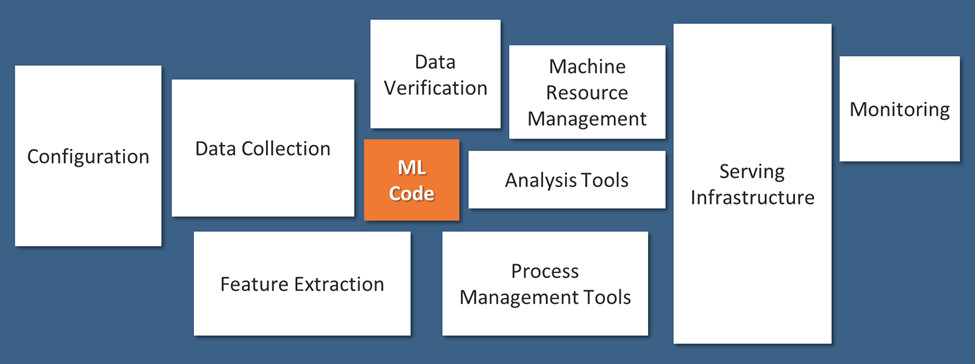
\includegraphics[scale=1]{imagenes/01_Introduccion/mlcodefraction.jpg}
	\centering
	\caption{Como se muestra en la figura, la fracción de código en los sistemas de ML reales es bastante pequeña. En cambio la fracción de infraestructura es mucho mayor \cite{bank2020autoencoders}.}
\end{figure}

En este caso, adoptar las mejores prácticas de \textbf{DevOps} (una metodología para desarrollo de software basada en la integración entre desarrolladores de software y administradores de sistemas) podría ser posible, pues el Machine Learning tiene mucho en común con la ingeniería del software. La diferencia es que en Machine Learning hay que llevar un registro de modelos y sus hiperparámetros, con el fin de que el experimento se pueda replicar con la mayor facilidad en otro sistema (esto recibe el nombre de reproducibilidad).\newline

En DevOps y MLOps se debe de usar un sistema de control de versiones (git) para poder gestionar los cambios en el código. Adicionalmente, en MLOps necesitamos versionar los modelos y sus hiperparámetros, pero gracias a la herramienta DVC (su uso está explicado en un capítulo posterior) esto ya no es problema. Además de todo lo anterior, el código debe de estar subido a un repositorio remoto compartido (como puede ser GitHub, GitLab, Bitbucket, etc) para poder trabajar cómodamente en equipo. En este repositorio debemos tener el control de que en cada cambio incremental todo lo anterior y lo nuevo siga funcionando, por lo tanto es necesario el uso de lo que se llama Integración Continua. Este proceso de Integración Continua lo que hace es ejecutar los tests que hemos escrito sobre el código implementado para comprobar que efectivamente funciona como esperábamos. En cuanto a MLOps, también es necesario testear que los modelos se comporten como esperamos. Esto nos permite desarrollar software de mayor calidad y con una altísima frecuencia de releases.\newline

Además de lo anterior, también se puede configurar un Despliegue Continuo, así si nuestro código pasa con éxito los tests de Integración Continua, podriamos desplegarlo en cuestión de segundos o unos pocos minutos mediante otras herramientas/plataformas que nos permitan acelerar dicho despliegue usando Infraestructura como Código. Para poder integrar la Integración Continua y el Despliegue Continuo (a partir de ahora lo llamaremos CI/CD) nos hace falta una plataforma en la nube que nos lo permita. Todo esto está desarrollado en los próximos capítulos de este documento.



%
%\input{capitulos/02_EspecificacionRequisitos}
%
%\input{capitulos/03_Planificacion}
%
%\input{capitulos/04_Analisis}
%
%\input{capitulos/05_Diseno}
%
%\input{capitulos/06_Implementacion}
%
%\input{capitulos/07_Pruebas}
%
%\chapter{Conclusiones y Trabajos Futuros}

\section{Conclusiones}

En este trabajo se ha intentado hacer una guía lo más completa posible del campo del \textit{Machine Learning} desde la perspectiva de la Ingeniería. En los capítulos anteriores se ha llegado a una solución usando las prácticas de \textit{DevOps} en el contexto del \textit{Machine Learning}, lo cual recibe el nombre de \textit{MLOps}. Sobre esto último no hay muchos trabajos publicados en internet.\\

La solución propuesta hace uso de contenedores y de software libre de tal forma que los experimentos y la infraestructura virtual usada en este trabajo son reproducibles por cualquier persona o entidad (usando la \textit{cloud} o incluso su propia infraestructura). Para poder reproducir lo anterior mencionado, se ha dejado una guía en el fichero \path{README.md} del repositorio de \textit{GitHub}.\\

Por otro lado, se ha conseguido unos resultados muy buenos en el problema que se pretendía resolver en este trabajo, llegando a un valor de 0.99 para la métrica $F_1$ en el conjunto de pruebas y además pudiendo analizar cuáles son los hiperparámetros que mayor efecto tienen sobre la métrica que mide la capacidad predictiva del modelo entrenado.\\

Gracias al uso de la herramienta \textit{mlflow} se ha podido llevar un \textit{tracking} de los experimentos, es decir, se ha podido guardar los hiperparámetros con los que se han entrenado los modelos y las métricas. Además, ha permitido almacenar automáticamente el modelo entrenado para su posterior descarga y despliegue en otra máquina y algunos \textit{plots} (como la matriz de confusión) para su posterior análisis. Y por último, mencionar la gran utilidad del framework \textit{SnapperML}, con el cual he podido definir los experimentos en ficheros con formato \textit{YAML} para poder ejecutar los experimentos fácilmente y guardar los resultados y artefactos en \textit{mlflow}.

\section{Trabajos Futuros}

Este trabajo constituye solo la primera parte de mi estudio sobre las técnicas de \textit{MLOps}, ya tengo listo el \textit{workflow} para entrenar modelos y he ideado como sería el despliegue del modelo en un microservicio y en el contexto del \textit{Edge Computing} (ver Capítulo \ref{chap:deploy}). Claramente, los siguientes pasos de este trabajo serían aprender sobre herramientas de orquestación para hacer pruebas de concepto de cómo sería el despliegue en el observatorio (o cualquier otro dentro del contexto del \textit{Edge Computing}), además de probar y añadir la infraestructura necesaria para monitorización y \textit{logging}.\\

Además, se podría adaptar el \textit{workflow} actual a \textit{kubernetes} para hacer que el despliegue de \textit{mlflow} y de los servicios que usa \textit{SnapperML} sea realizado con una única orden y por tanto de forma más sencilla. Por último, recalcar que también sería interesante implementar \textit{tests} de infraestructura para comprobar que la infraestructura levantada funciona tal y como está planificado que lo haga.\\

%
%%\chapter{Conclusiones y Trabajos Futuros}
%
%
%%\nocite{*}
%\bibliography{bibliografia/bibliografia}\addcontentsline{toc}{chapter}{Bibliografía}
%\bibliographystyle{miunsrturl}
%
%\appendix
%\input{apendices/manual_usuario/manual_usuario}
%\input{glosario/entradas_glosario}
% \addcontentsline{toc}{chapter}{Glosario}
% \printglossary
\chapter*{}
\thispagestyle{empty}

\end{document}
